\chapter{Gelombang pada Tali dan Batang: Persamaan d'Alembert}\label{ch:b2:waves-on-strings}

Petiklah senar gitar dan sebuah bentuk berlari sepanjangnya, memantul di
jembatannya, kembali, lalu menetap menjadi pola berdiri yang
frekuensinya Anda dengar sebagai sebuah nada. Tempelkanlah telinga Anda
pada rel kereta dan Anda mendengar keretanya jauh sebelum ia tiba: sebuah
mampatan berlari menyusuri bajanya pada lima kilometer tiap sekon. Jilid
Tahun ke-1 melukiskan gelombang semacam itu --- berjalan, berdiri,
tertumpangkan --- tanpa mengatakan mengapa ia ada. Bab ini menurunkan
persamaan yang mengaturnya, \emph{\omterm{thm:b2:waves-on-strings:equation}{persamaan gelombang} d'Alembert},
mula-mula bagi gerak transversal sebuah tali, lalu bagi gerak
longitudinal sebuah batang yang dibangun, atom demi atom, dari massa dan
pegas; bab ini menghitung energi yang diemban sebuah gelombang dan
impedansi yang memutuskan apa yang terjadi ketika ia menjumpai perubahan
medium.

\section{Tali yang bergetar}

\begin{theorem}[Persamaan gelombang sebuah tali]\label{thm:b2:waves-on-strings:equation}
\index{persamaan d'Alembert}\index{persamaan gelombang}\index{kelajuan gelombang (tali)}
Sebuah tali berapat massa linear $\mu$, yang teregang dengan tegangan $T$,
membuat simpangan transversal kecil $y(x, t)$ (kemiringan $|\partial_xy| \ll 1$). Maka
\[
\frac{\partial^2y}{\partial t^2} = c^2\,\frac{\partial^2y}{\partial x^2} ,
\qquad c = \sqrt{\frac{T}{\mu}} ,
\]
yaitu \emph{\omterm{thm:b2:waves-on-strings:equation}{persamaan d'Alembert}}, yang penyelesaian umumnya adalah $y = f(x - ct)
+ g(x + ct)$: tumpangan sebuah bentuk yang berjalan ke kanan dan
satu lagi yang berjalan ke kiri dengan kelajuan $c$, tanpa berubah bentuk.
\end{theorem}

\begin{proof}
Kucilkanlah unsur antara $x$ dan $x + \dd x$, bermassa $\mu\,\dd x$.
Tetangganya menariknya sepanjang garis singgung talinya dengan tegangan $T$:
secara mendatar $T\cos\theta \approx T$ di kedua ujungnya (tak ada gerak mendatar, jadi
$T$ sama di sepanjangnya), secara tegak $T\sin\theta \approx T\partial_xy$, yang
memberi gaya total $T[\partial_xy(x + \dd x) - \partial_xy(x)] = T\,\partial_x^2y\,\dd x$.
Newton: $\mu\,\dd x\,\partial_t^2y = T\partial_x^2y\,\dd x$. Untuk penyelesaiannya, misalkan
$u = x - ct$, $v = x + ct$: persamaannya menjadi $\partial_u\partial_vy = 0$
(aturan rantai), jadi $\partial_vy$ hanya bergantung pada $v$, dan $y = f(u) + g(v)$;
sebaliknya sembarang $y$ semacam itu memenuhinya. Gravitasi, yang diabaikan, sah
diabaikan bila $T \gg \mu gL$.
\end{proof}

\begin{omfigure}
\begin{tikzpicture}[font=\small, x=1cm, y=1cm, >=Stealth]
  \begin{scope}
    \draw[->] (-2.5,0) -- (3.0,0) node[right, font=\footnotesize] {$x$};
    \draw[omDef, very thick, domain=-2.3:2.8, samples=60] plot (\x,{0.9*exp(-(\x)^2/1.6)});
    \coordinate (A) at (-0.6,{0.9*exp(-0.36/1.6)}); \coordinate (B) at (0.2,{0.9*exp(-0.04/1.6)});
    \fill[omThm] (A) circle (1.5pt); \fill[omThm] (B) circle (1.5pt);
    \draw[omThm, very thick, ->] (A) -- ($(A)+(-0.9,-0.55)$) node[above left, font=\footnotesize, yshift=2pt] {$\vect T(x)$};
    \draw[omThm, very thick, ->] (B) -- ($(B)+(1.0,-0.12)$) node[right, font=\footnotesize] {$\vect T(x+\dd x)$};
    \draw[dashed] (-0.6,0) -- (A); \draw[dashed] (0.2,0) -- (B);
    \node[font=\footnotesize] at (-0.6,-0.3) {$x$}; \node[font=\footnotesize] at (0.35,-0.3) {$x + \dd x$};
    \node[font=\footnotesize] at (0.2,-0.9) {$\mu\,\dd x\,\partial_t^2y = T\,\partial_x^2y\,\dd x$};
  \end{scope}
  \begin{scope}[xshift=7.6cm]
    \draw[->] (-2.5,0) -- (3.0,0) node[right, font=\footnotesize] {$x$};
    \draw[omDef, thick, domain=-2.3:2.8, samples=60] plot (\x,{0.8*exp(-(\x+1.3)^2/0.5)});
    \draw[omDef, thick, dashed, domain=-2.3:2.8, samples=60] plot (\x,{0.8*exp(-(\x-0.5)^2/0.5)});
    \draw[omDef, thick, ->] (-1.0,1.0) -- (0.2,1.0) node[above, font=\footnotesize, pos=0.5] {$c$};
    \node[font=\footnotesize] at (-1.3,-0.35) {$t$}; \node[font=\footnotesize] at (0.5,-0.35) {$t + \tau$};
    \node[font=\footnotesize] at (0.2,-0.9) {$y = f(x - ct)$};
  \end{scope}
\end{tikzpicture}

{\small Kiri: gaya-gaya pada sebuah unsur tali --- kedua tegangannya
tidak sejajar ketika talinya melengkung, dan resultannya bersifat
transversal. Kanan: sebuah bentuk $f(x - ct)$ berjalan ke kanan dengan $c$
tanpa berubah bentuk.}
\end{omfigure}

\begin{example}[Gitar, piano, kabel]\label{ex:b2:waves-on-strings:numbers}
Senar E rendah sebuah gitar ($\mu = \qty{5.5}{g/m}$, panjang \qty{0.65}{m},
\qty{82.4}{Hz}) bergetar pada nada dasarnya dengan $\lambda = 2L$: $c = 2Lf =
\qty{107}{m/s}$ dan $T = \mu c^2 = \qty{63}{N}$. Dawai A$_4$ sebuah piano (baja,
\qty{1}{mm}, $\mu = \qty{6.1}{g/m}$, \qty{0.38}{m}, \qty{440}{Hz}): $c = \qty{334}{m/s}$,
$T = \qty{680}{N}$ --- dan ada sekitar $230$ dawai dalam sebuah piano, dua puluh
ton tegangan pada rangka besi tuangnya. Kabel \qty{1}{kg/m} pada \qty{10}{kN}:
\qty{100}{m/s}.
\end{example}

\section{Gelombang berdiri dan ragam getar}

\begin{proposition}[Ragam sebuah tali yang terikat di kedua ujungnya]\label{prop:b2:waves-on-strings:modes}
\index{ragam normal}\index{harmonik}\index{gelombang berdiri}
Sebuah tali yang terikat di $x = 0$ dan $x = L$ menerima penyelesaian
\omterm{prop:b2:waves-on-strings:modes}{gelombang berdiri} sinusoidal (\emph{\omterm{prop:b2:waves-on-strings:modes}{ragam normal}})
\[
y_n(x, t) = A_n\sin\frac{n\pi x}{L}\cos(\omega_nt - \varphi_n) , \qquad
f_n = \frac{\omega_n}{2\pi} = n\,\frac{c}{2L} = n f_1 , \quad n = 1, 2, 3, \dots
\]
--- yaitu nada dasar $f_1 = c/2L$ dan \emph{harmonik}nya. Ragam $n$ mempunyai
$n - 1$ simpul di antara kedua ujungnya. Setiap gerak talinya adalah
tumpangan $y = \sum_ny_n$, dengan amplitudo dan fasenya ditetapkan oleh
bentuk dan kecepatan awalnya (sebuah deret Fourier, sebagaimana ditegakkan
jilid matematika tahun ini): campuran harmoniknya adalah
\emph{warna bunyi} nadanya.
\end{proposition}

\begin{proof}
Carilah $y = F(x)\cos(\omega t - \varphi)$: $F'' + (\omega/c)^2F = 0$, $F(0) = 0$ memberi
$F = A\sin(\omega x/c)$, dan $F(L) = 0$ menuntut $\omega L/c = n\pi$. Setiap ragam juga
merupakan jumlah dua gelombang berjalan: $\sin kx\cos\omega t = \tfrac12[\sin(kx -
\omega t) + \sin(kx + \omega t)]$ --- gelombangnya dan pantulannya.
Kelengkapan sinusnya adalah teorema Fourier.
\end{proof}

\begin{omfigure}
\begin{tikzpicture}
\begin{axis}[omaxis, axis x line=bottom, axis y line=none, width=6.4cm, height=5.2cm,
    xmin=0, xmax=1, ymin=-5.9, ymax=1.5, xtick={0,1}, xticklabels={$0$, $L$}, samples=80,
    xlabel={}, ylabel={}]
  \addplot[omDef, thick, domain=0:1] {sin(deg(pi*x))};
  \addplot[omDef, thick, dashed, domain=0:1] {-sin(deg(pi*x))};
  \addplot[omThm, thick, domain=0:1] {0.8*sin(deg(2*pi*x))-2.6};
  \addplot[omThm, thick, dashed, domain=0:1] {-0.8*sin(deg(2*pi*x))-2.6};
  \addplot[omProp, thick, domain=0:1] {0.7*sin(deg(3*pi*x))-5.0};
  \addplot[omProp, thick, dashed, domain=0:1] {-0.7*sin(deg(3*pi*x))-5.0};
  \addplot[black, thin] coordinates {(0,-2.6) (1,-2.6)};
  \addplot[black, thin] coordinates {(0,-5.0) (1,-5.0)};
  \node[font=\scriptsize] at (axis cs:0.5,1.25) {$n = 1$};
  \node[font=\scriptsize] at (axis cs:0.5,-1.4) {$n = 2$};
  \node[font=\scriptsize] at (axis cs:0.5,-3.85) {$n = 3$};
\end{axis}
\end{tikzpicture}
\hfill
\begin{tikzpicture}
\begin{axis}[omaxis, axis x line=bottom, axis y line=left, width=5.0cm, height=4.2cm,
    xlabel={$x/L$}, ylabel={$y$}, xmin=0, xmax=1, ymin=-0.05, ymax=1.1, xtick={0,0.5,1}, ytick=\empty, samples=200, clip=false,
    xlabel style={at={(axis description cs:0.5,-0.12)}, anchor=north},
    ylabel style={at={(axis description cs:-0.06,0.5)}, rotate=90, anchor=south}]
  \addplot[black, thick] coordinates {(0,0) (0.5,1) (1,0)};
  \addplot[omDef, thick, domain=0:1] {0.81*sin(deg(pi*x))};
  \addplot[omThm, thick, domain=0:1] {0.81*sin(deg(pi*x)) - 0.09*sin(deg(3*pi*x))};
  \node[font=\scriptsize, anchor=west] at (axis cs:0.03,0.95) {dipetik};
  \node[font=\scriptsize, omDef, anchor=east] at (axis cs:0.97,0.95) {$n = 1$};
  \node[font=\scriptsize, omThm, anchor=east] at (axis cs:0.97,0.78) {$n = 1, 3$};
\end{axis}
\end{tikzpicture}

{\small Kiri: ketiga ragam pertama sebuah tali yang terikat di kedua ujungnya ($f_n = nc/2L$).
Kanan: sebuah tali yang dipetik di tengahnya (segitiga) dan suku-suku pertama
deret Fouriernya --- hanya harmonik ganjil yang muncul, dengan amplitudo
yang turun sebagai $1/n^2$.}
\end{omfigure}

\begin{example}[Percobaan Melde]\label{ex:b2:waves-on-strings:melde}
\index{percobaan Melde}
Sebuah tali yang digetarkan di satu ujungnya oleh sebuah vibrator berfrekuensi $f$, dengan ujung lainnya
melewati katrol menuju massa gantung $m$ (sehingga $T = mg$): sebuah
\omterm{prop:b2:waves-on-strings:modes}{gelombang berdiri} yang besar muncul setiap kali $f$ sama dengan salah satu $f_n = (n/2L)
\sqrt{mg/\mu}$ --- resonansi ragam $n$. Untuk $L = \qty{1.2}{m}$, $\mu =
\qty{1.0}{g/m}$ dan $f = \qty{50}{Hz}$, massa yang memberi $n = 1, 2, 3$ perut
adalah $m_n = 4L^2f^2\mu/n^2g = 1.47/n^2$ kg: \qty{1.47}{kg}, \qty{367}{g}, \qty{163}{g}.
Menekan senar gitar pada fret kedua belas memisahduakan $L$ dan melipatduakan
$f_1$: oktafnya; menyentuhnya ringan di tengah tanpa menekan
mematikan ragam ganjilnya dan menyisakan harmonik kedua --- flageoletnya.
\end{example}

\section{Energi, daya dan impedansi}

\begin{proposition}[Energi gelombang pada tali]\label{prop:b2:waves-on-strings:energy}
\index{rapat energi (tali)}\index{fluks energi (tali)}\index{impedansi (tali)}
Sebuah tali mengemban energi tiap satuan panjang dan daya (fluks
energi menuju $+x$)
\[
e = \tfrac12\mu\Bigl(\frac{\partial y}{\partial t}\Bigr)^2 + \tfrac12T\Bigl(\frac{\partial y}{\partial x}\Bigr)^2 ,
\qquad
\mathcal P = -T\,\frac{\partial y}{\partial x}\,\frac{\partial y}{\partial t} ,
\]
yang menuruti neraca lokal $\partial_te + \partial_x\mathcal P = 0$. Bagi
gelombang berjalan $y = f(x - ct)$, rapat kinetik dan potensialnya
sama dan $\mathcal P = Z\,(\partial_ty)^2$ dengan
\[
Z = \sqrt{T\mu} = \mu c = \frac Tc ,
\]
yaitu \emph{impedansi} talinya (\unit{kg/s}): nisbah antara
gaya transversal $-T\partial_xy$ yang dikerahkan talinya pada apa yang ada di depannya
dan kecepatan transversal $\partial_ty$. Gelombang sinusoidal beramplitudo $A$
mengemban daya rerata $\langle\mathcal P\rangle = \tfrac12Z\omega^2A^2$.
\end{proposition}

\begin{proof}
Suku potensialnya adalah usaha tegangan yang meregangkan unsurnya:
panjangnya adalah
\[
\dd x\sqrt{1 + (\partial_xy)^2} \approx \dd x\bigl(1 + \tfrac12(\partial_xy)^2\bigr) ,
\]
jadi kelebihan panjangnya dikali $T$ memberi $\tfrac12T(\partial_xy)^2\dd x$. Daya
yang disalurkan menyeberangi $x$ menuju $+x$ adalah gaya transversal yang dikerahkan
bagian kirinya pada bagian kanannya, $-T\partial_xy$, dikali kecepatannya
$\partial_ty$. Neracanya:
\[
\partial_te = \mu\,\partial_ty\,\partial_t^2y + T\,\partial_xy\,\partial_x\partial_ty ,
\qquad
-\partial_x\mathcal P = T\,\partial_x^2y\,\partial_ty + T\,\partial_xy\,\partial_x\partial_ty ,
\]
yang sama menurut \omterm{thm:b2:waves-on-strings:equation}{persamaan gelombangnya}. Bagi $f(x - ct)$: $\partial_xy = -\partial_ty/c$, jadi $\mathcal P = (T/c)
(\partial_ty)^2$ dan kedua rapatnya sama dengan $\tfrac12\mu(\partial_ty)^2$.
\end{proof}

\begin{proposition}[Pemantulan dan penerusan di sebuah sambungan]\label{prop:b2:waves-on-strings:junction}
\index{koefisien pemantulan (tali)}\index{koefisien penerusan (tali)}
Sebuah gelombang beramplitudo $A_i$ tiba dari tali berimpedansi $Z_1$ pada
tali berimpedansi $Z_2$ yang tersambung di $x = 0$. Kesinambungan
simpangan dan gaya transversal di sambungannya memberi
koefisien amplitudo
\[
r = \frac{A_r}{A_i} = \frac{Z_1 - Z_2}{Z_1 + Z_2} , \qquad
t = \frac{A_t}{A_i} = \frac{2Z_1}{Z_1 + Z_2} ,
\]
dan bagian energinya $R = r^2$, $\mathcal T = 4Z_1Z_2/(Z_1 + Z_2)^2$, dengan
$R + \mathcal T = 1$. Ujung tetap ($Z_2 \to \infty$) memantulkan dengan $r = -1$
(pulsanya kembali terbalik), ujung bebas ($Z_2 = 0$) dengan $r = +1$;
impedansi yang sama meneruskan segalanya.
\end{proposition}

\begin{proof}
Gelombang sinusoidal $y_1 = A_i\cos(\omega t - k_1x) + A_r\cos(\omega t + k_1x)$ untuk
$x < 0$, $y_2 = A_t\cos(\omega t - k_2x)$ untuk $x > 0$, dengan $\omega$ yang sama di kedua
sisinya. Di $x = 0$: $y_1 = y_2$ memberi $A_i + A_r = A_t$; gayanya $-T\partial_xy$
yang sinambung (sambungan tanpa massa) memberi $Z_1(A_i - A_r) = Z_2A_t$ (dengan memakai
$T_1k_1 = Z_1\omega$). Selesaikanlah. Energinya: daya rerata $\tfrac12Z\omega^2A^2$.
\end{proof}

\begin{omfigure}
\begin{tikzpicture}[font=\small, x=1cm, y=1cm, >=Stealth]
  \begin{scope}
    \draw[->] (-3.2,0) -- (3.2,0) node[right, font=\footnotesize] {$x$};
    \draw[omDef, very thick, domain=-3.0:0, samples=50] plot (\x,{0.8*exp(-(\x+1.6)^2/0.25)});
    \draw[omDef, very thick, domain=0:3.0, samples=50] plot (\x,{0});
    \fill (0,0) circle (2pt); \node[font=\footnotesize] at (0,-0.35) {$Z_1 \to Z_2$};
    \draw[omDef, ->, thick] (-1.6,1.0) -- (-0.8,1.0) node[above, font=\footnotesize, pos=0.5] {$A_i$};
    \node[font=\footnotesize] at (-1.5,-0.6) {$Z_1$}; \node[font=\footnotesize] at (1.5,-0.6) {$Z_2 > Z_1$};
    \node[font=\footnotesize] at (0,-1.1) {sebelum};
  \end{scope}
  \begin{scope}[xshift=7.2cm]
    \draw[->] (-3.2,0) -- (3.2,0) node[right, font=\footnotesize] {$x$};
    \draw[omThm, very thick, domain=-3.0:0, samples=50] plot (\x,{-0.27*exp(-(\x+1.6)^2/0.25)});
    \draw[omProp, very thick, domain=0:3.0, samples=50] plot (\x,{0.53*exp(-(\x-1.1)^2/0.12)});
    \fill (0,0) circle (2pt);
    \draw[omThm, ->, thick] (-1.0,0.5) -- (-1.8,0.5) node[above, font=\footnotesize, pos=0.5] {$rA_i$};
    \draw[omProp, ->, thick] (1.0,0.9) -- (1.8,0.9) node[above, font=\footnotesize, pos=0.5] {$tA_i$};
    \node[font=\footnotesize] at (0,-1.1) {sesudah: $r = \dfrac{Z_1 - Z_2}{Z_1 + Z_2}$, $t = \dfrac{2Z_1}{Z_1 + Z_2}$};
  \end{scope}
\end{tikzpicture}

{\small Sebuah pulsa menjumpai sambungan dengan tali yang lebih berat ($Z_2 = 4Z_1$):
sebagian diteruskan, lebih lambat dan lebih sempit, sebagian dipantulkan terbalik.}
\end{omfigure}

\section{Dari rantai atom ke batang elastik}

\begin{proposition}[Rantai atom; modulus Young]\label{prop:b2:waves-on-strings:chain}
\index{rantai atom}\index{modulus Young}\index{hukum Hooke}\index{gelombang longitudinal}
Sebuah barisan massa serupa $m$ yang berjarak $a$ dan tersambung oleh pegas
berkekakuan $k$: jika $u_n(t)$ adalah simpangan massa ke-$n$ sepanjang
barisannya,
\[
m\ddot u_n = k(u_{n+1} - u_n) - k(u_n - u_{n-1}) = k(u_{n+1} - 2u_n + u_{n-1}) .
\]
Ketika simpangannya berubah perlahan dari satu massa ke massa berikutnya (pada
panjang gelombang $\lambda \gg a$), $u_n(t) \to u(x, t)$ dengan $u_{n\pm1} - u_n \approx
\pm a\,\partial_xu + \tfrac12a^2\partial_x^2u$, dan rantainya menuruti \omterm{thm:b2:waves-on-strings:equation}{persamaan
d'Alembert}
\[
\frac{\partial^2u}{\partial t^2} = c^2\frac{\partial^2u}{\partial x^2} , \qquad
c = a\sqrt{\frac km} = \sqrt{\frac{E}{\rho}} ,
\]
dengan $\rho = m/a^3$ massa jenis zat padat yang tersusun atas rantai semacam itu dalam
susunan kubus dan $E = k/a$ \emph{\omterm{prop:b2:waves-on-strings:chain}{modulus Young}}nya: kekakuan
sebuah batang berpenampang $S$ dan sepanjang $\ell$ adalah $kS/a^2\cdot a/\ell = ES/\ell$,
yakni \emph{\omterm{prop:b2:waves-on-strings:chain}{hukum Hooke}} $F/S = E\,\Delta\ell/\ell$ (tegangan $\sigma = E\varepsilon$).
\end{proposition}

\begin{proof}
Tiap pegas teregang sebesar selisih simpangan kedua
ujungnya. Sisipkanlah uraian Taylornya: $m\partial_t^2u = ka^2\partial_x^2u$. Sebuah kubus
bersisi $a$ tiap atom memberi $\rho = m/a^3$; batang berpenampang $S$ memuat
$S/a^2$ rantai sejajar yang berisi $\ell/a$ pegas terseri, dengan kekakuan total
$(S/a^2)(ka/\ell) = (k/a)S/\ell$.
\end{proof}

\begin{proposition}[Gelombang longitudinal dalam sebuah batang]\label{prop:b2:waves-on-strings:rod}
\index{bunyi dalam zat padat}
Langsung pada kontinumnya: sebuah unsur batang antara $x$ dan $x +
\dd x$, yang tersimpangkan sebesar $u(x, t)$, teregang sebesar $\varepsilon = \partial_xu$ dan tertarik
oleh tegangan $\sigma = E\partial_xu$ pada tiap mukanya; Newton memberi $\rho\,\partial_t^2u =
E\,\partial_x^2u$: \omterm{prop:b2:waves-on-strings:chain}{gelombang longitudinal} (mampatan) berjalan dengan $c = \sqrt{E/\rho}$
--- \qty{5100}{m/s} dalam baja ($E = \qty{200}{GPa}$), \qty{5000}{m/s} dalam aluminium,
\qty{3700}{m/s} dalam granit, \qty{3500}{m/s} dalam kayu searah seratnya.
Impedansinya adalah $Z = \rho c = \sqrt{E\rho}$ tiap satuan luas, dan rumus
sambungan yang sama berlaku --- itulah cara ultrasonik menemukan retakan pada
sebuah rel.
\end{proposition}

\begin{proof}
Gaya total pada unsurnya: $S[\sigma(x + \dd x) - \sigma(x)] = SE\partial_x^2u\,\dd x$;
massanya $\rho S\dd x$.
\end{proof}

\begin{omfigure}
\begin{tikzpicture}[font=\small, x=1cm, y=1cm, >=Stealth]
  \begin{scope}
    \foreach \i in {0,1,2,3,4} {
      \fill[omDef] ({1.4*\i},0) circle (5pt);
    }
    \foreach \i in {0,1,2,3} {
      \draw[thick, decorate, decoration={coil, aspect=0.5, segment length=4pt, amplitude=3pt}] ({1.4*\i+0.18},0) -- ({1.4*\i+1.22},0);
    }
    \node[font=\footnotesize] at (1.4,-0.5) {$u_{n-1}$}; \node[font=\footnotesize] at (2.8,-0.5) {$u_n$}; \node[font=\footnotesize] at (4.2,-0.5) {$u_{n+1}$};
    \draw[<->] (1.4,0.45) -- (2.8,0.45) node[midway, above, font=\footnotesize] {$a$};
    \node[font=\footnotesize] at (2.8,-1.1) {$m\ddot u_n = k(u_{n+1} - 2u_n + u_{n-1})$};
  \end{scope}
  \begin{scope}[xshift=8.0cm]
    \draw[thick] (-2.0,-0.5) rectangle (2.6,0.5);
    \fill[omDef!25] (-0.3,-0.5) rectangle (0.5,0.5);
    \draw[omThm, very thick, ->] (-0.3,0) -- (-1.2,0) node[above, font=\footnotesize, pos=0.6] {$\sigma(x)S$};
    \draw[omThm, very thick, ->] (0.5,0) -- (1.5,0) node[above, font=\footnotesize, pos=0.6] {$\sigma(x + \dd x)S$};
    \node[font=\footnotesize] at (0.1,-0.8) {$\rho S\dd x\,\partial_t^2u = SE\,\partial_x^2u\,\dd x$};
    \node[font=\footnotesize] at (0.3,-1.35) {$c = \sqrt{E/\rho}$};
  \end{scope}
\end{tikzpicture}

{\small Kiri: rantai massa dan pegas --- tiap massa merasakan
kedua pegas di sekitarnya, dan limit kontinumnya adalah \omterm{thm:b2:waves-on-strings:equation}{persamaan gelombang}
dengan $c = a\sqrt{k/m}$. Kanan: sebuah unsur batang elastik yang ditarik
tegangan pada kedua mukanya.}
\end{omfigure}

\begin{remark}[Apa yang diketahui rantainya dan tidak diketahui batangnya]\label{rem:b2:waves-on-strings:dispersion}
Mencari $u_n = A\cos(\omega t - kna)$ dalam persamaan rantai yang eksak memberi
$\omega = 2\sqrt{k/m}\,|\sin(ka/2)|$: untuk $ka \ll 1$ ini adalah $\omega = ck$, yaitu
\omterm{thm:b2:waves-on-strings:equation}{persamaan gelombang} tanpa dispersi, tetapi ketika panjang gelombangnya mendekati $2a$
frekuensinya jenuh pada $2\sqrt{k/m}$ dan kecepatan fase serta kecepatan grupnya
berbeda --- \emph{hubungan dispersi} pertama dalam jilid ini, yang menjadi
pokok \cref{ch:b2:dispersion-wave-packets}. Untuk $a = \qty{0.25}{nm}$ dan
$c = \qty{5}{km/s}$ ambang atasnya terletak di $\omega_{\max} = 2c/a = \qty{4e13}{rad/s}$
(\qty{6}{THz}): zat padatnya tak dapat bergetar lebih cepat daripada yang diizinkan
pegas atomnya.
\end{remark}

\section{Latihan}

\begin{exercise}[$\star$]\label{exo:b2:waves-on-strings:1}
Senar A sebuah gitar (\qty{110}{Hz}, $L = \qty{65}{cm}$, $\mu = \qty{3.0}{g/m}$):
tentukanlah kelajuan gelombangnya, tegangannya, panjang gelombang nada dasarnya pada senarnya dan
panjang gelombang bunyinya di udara; frekuensinya ketika senarnya ditekan pada fret
kelima ($L$ berkurang dengan faktor $2^{-5/12}$).
\end{exercise}

\begin{exercise}[$\star$]\label{exo:b2:waves-on-strings:2}
Kelajuan \omterm{prop:b2:waves-on-strings:chain}{gelombang longitudinal} dalam baja ($E = \qty{200}{GPa}$, $\rho =
\qty{7800}{kg/m^3}$), aluminium (\qty{70}{GPa}, \qty{2700}{kg/m^3}) dan timbal
(\qty{16}{GPa}, \qty{11300}{kg/m^3}). Waktu bagi bunyi untuk menempuh \qty{1.0}{km}
sepanjang rel dan lewat udara (\qty{340}{m/s}); apa yang didengar seorang pendengar
yang menempelkan telinganya pada rel.
\end{exercise}

\begin{exercise}[$\star$]\label{exo:b2:waves-on-strings:3}
Sebuah tali bernada dasar \qty{200}{Hz}: frekuensi dan jumlah simpul
ragam 2, 3, 4; kedudukan simpul ragam 3; frekuensi
nada dasarnya jika tegangannya dilipatduakan, jika panjangnya dipisahduakan, jika
talinya diganti dengan tali tiga kali lebih berat tiap meter.
\end{exercise}

\begin{exercise}[$\star$]\label{exo:b2:waves-on-strings:4}
Sebuah tambang \qty{12}{m} ($\mu = \qty{0.20}{kg/m}$) ditarik dengan \qty{45}{N}; satu
ujungnya diikatkan ke dinding. Sebuah pulsa dikirim dari ujung lainnya. Tentukanlah kelajuannya;
waktu untuk mencapai dinding dan kembali; bentuk pulsa yang kembali;
hal yang sama jika ujung jauhnya diikat pada cincin ringan yang meluncur bebas pada
sebuah tiang.
\end{exercise}

\begin{exercise}[$\star\star$]\label{exo:b2:waves-on-strings:5}
Sebuah dawai piano bagi \qty{440}{Hz}: baja ($\rho = \qty{7800}{kg/m^3}$),
berdiameter \qty{1.0}{mm}, panjang berbunyi \qty{38}{cm}. (a) $\mu$, kelajuan gelombangnya,
tegangannya. (b) Tegangan tarik dalam kawatnya; bandingkanlah dengan kekuatan kawat
piano, sekitar \qty{2}{GPa}. (c) Nada yang sama dengan kawat \qty{0.5}{mm}: tegangan tali
dan tegangan tariknya. (d) Mengapa dawai bas dililit tembaga alih-alih dibuat
lebih panjang atau lebih tebal?
\end{exercise}

\begin{exercise}[$\star\star$]\label{exo:b2:waves-on-strings:6}
\emph{Melde.} Sebuah tali \qty{1.5}{m} ($\mu = \qty{2.0}{g/m}$) digetarkan pada
\qty{60}{Hz}; tegangannya ditetapkan sebuah massa gantung. (a) Massa yang memberi
$1$, $2$, $3$ dan $4$ perut. (b) Dengan \qty{0.50}{kg}: adakah resonansi?
Ragam terdekatnya. (c) Ujung yang digetarkan itu sebenarnya simpul atau perut?
(d) Mengapa perutnya tumbuh begitu besar saat resonansi, dan apa yang membatasinya?
\end{exercise}

\begin{exercise}[$\star\star$]\label{exo:b2:waves-on-strings:7}
Sebuah gelombang $y = A\cos(\omega t - kx)$ dengan $A = \qty{2.0}{mm}$, $f = \qty{100}{Hz}$
berjalan pada sebuah tali ($T = \qty{100}{N}$, $\mu = \qty{10}{g/m}$). Tentukanlah kelajuannya, $k$,
panjang gelombangnya; kecepatan dan percepatan transversal maksimum sebuah titik;
kemiringan maksimumnya; impedansinya; daya rerata yang diembannya; energi yang termuat dalam satu
panjang gelombang.
\end{exercise}

\begin{exercise}[$\star\star$]\label{exo:b2:waves-on-strings:8}
Sebuah tali $\mu_1 = \qty{2.0}{g/m}$ diikatkan pada tali $\mu_2 = \qty{8.0}{g/m}$,
keduanya di bawah \qty{20}{N}. (a) Kelajuan dan impedansinya. (b) Koefisien
pemantulan dan penerusan amplitudo bagi gelombang yang datang dari
tali ringannya; dari tali beratnya. (c) Bagian energinya dalam kedua
halnya; periksalah bahwa jumlahnya satu. (d) Sebuah pulsa setinggi \qty{1}{cm} dan selebar \qty{10}{cm}
tiba dari tali ringannya: tinggi dan lebar pulsa yang diteruskan dan
yang dipantulkan.
\end{exercise}

\begin{exercise}[$\star\star$]\label{exo:b2:waves-on-strings:9}
Sebuah kawat baja \qty{2.0}{m} berdiameter \qty{1.0}{mm} memanjang \qty{1.0}{mm}
di bawah \qty{80}{N}. (a) \omterm{prop:b2:waves-on-strings:chain}{Modulus Young}. (b) Kelajuan \omterm{prop:b2:waves-on-strings:chain}{gelombang longitudinal}.
(c) Frekuensi dasar getaran longitudinal kawatnya ketika ia
dijepit di kedua ujungnya, dan frekuensi getaran transversalnya di bawah tegangan itu;
mengapa keduanya begitu berbeda? (d) Kekakuan $k$ dan massa $m$ sebuah
``atom'' dalam model rantainya, untuk $a = \qty{0.25}{nm}$.
\end{exercise}

\begin{exercise}[$\star\star\star$]\label{exo:b2:waves-on-strings:10}
\emph{Tali yang dipetik.} Sebuah tali yang terikat di $0$ dan $L$ ditarik ke samping
di $x = L/2$ sampai ketinggian $h$ (bentuk segitiga) lalu dilepaskan dari keadaan diam.
(a) Tuliskanlah penyelesaiannya sebagai $\sum_nb_n\sin(n\pi x/L)\cos(\omega_nt)$ lalu tunjukkanlah
bahwa $b_n = \dfrac{8h}{n^2\pi^2}\sin\dfrac{n\pi}2$. (b) Harmonik mana yang
lenyap dan mengapa? (c) Energi ragam $n$ ($E_n = \tfrac14\mu L\omega_n^2b_n^2$);
bagian energi total yang ada pada nada dasarnya. (d) Talinya dipetik di
$L/5$ sebagai gantinya: harmonik mana yang lenyap? Mengapa seorang pemain gitar memetik dekat
jembatannya untuk bunyi yang lebih cerah?
\end{exercise}

\begin{exercise}[$\star\star\star$]\label{exo:b2:waves-on-strings:11}
\emph{Dispersi rantainya.} (a) Sisipkanlah $u_n = A\cos(\omega t - kna)$ dalam
persamaan rantainya lalu turunkanlah $\omega(k) = 2\omega_0|\sin(ka/2)|$, $\omega_0 =
\sqrt{k/m}$. (b) Kecepatan fase $\omega/k$ dan kecepatan grup $\dd\omega/\dd k$;
limit bersamanya untuk $ka \to 0$; nilainya pada $ka = \pi$. (c) Seperti apa
rupa gelombangnya pada $ka = \pi$? Mengapa tak ada gelombang yang
panjang gelombangnya lebih pendek daripada $2a$? (d) Untuk baja ($c = \qty{5.1}{km/s}$, $a =
\qty{0.25}{nm}$): $\omega_0$, frekuensi maksimumnya, dan panjang gelombang ultrasonik
\qty{1}{MHz} --- berdispersikah ia?
\end{exercise}

\begin{exercise}[$\star\star\star$]\label{exo:b2:waves-on-strings:12}
\emph{Tambang tergantung, cambuk yang meletup.} (a) Sebuah tambang serbasama sepanjang $L$
tergantung dari langit-langit: tegangannya pada ketinggian $x$ di atas ujung bebasnya;
kelajuan gelombang setempat $c(x)$. (b) Waktu bagi sebuah pulsa untuk menempuh dari bawah ke
atas; angkanya untuk $L = \qty{10}{m}$; mengapa bentuk pulsanya berubah. (c) Sebuah
cambuk meruncing, dengan $\mu$ yang mengecil menuju ujungnya, pada tegangan yang (hampir)
tetap selama sabetannya: bagaimana kelajuannya berubah sepanjangnya? (d)
Dengan menerima bahwa energi pulsanya kekal dan durasinya
tetap, tunjukkanlah bahwa amplitudo kecepatan transversalnya
tumbuh sebagai $\mu^{-1/4}$, lalu perkirakanlah kelajuan ujung sebuah cambuk yang
$\mu$-nya turun dengan faktor $10^4$ dari gagang ke ujungnya jika tangannya memberi
\qty{10}{m/s}. (Letupannya adalah ledakan sonik.)
\end{exercise}

\begin{omfigure}
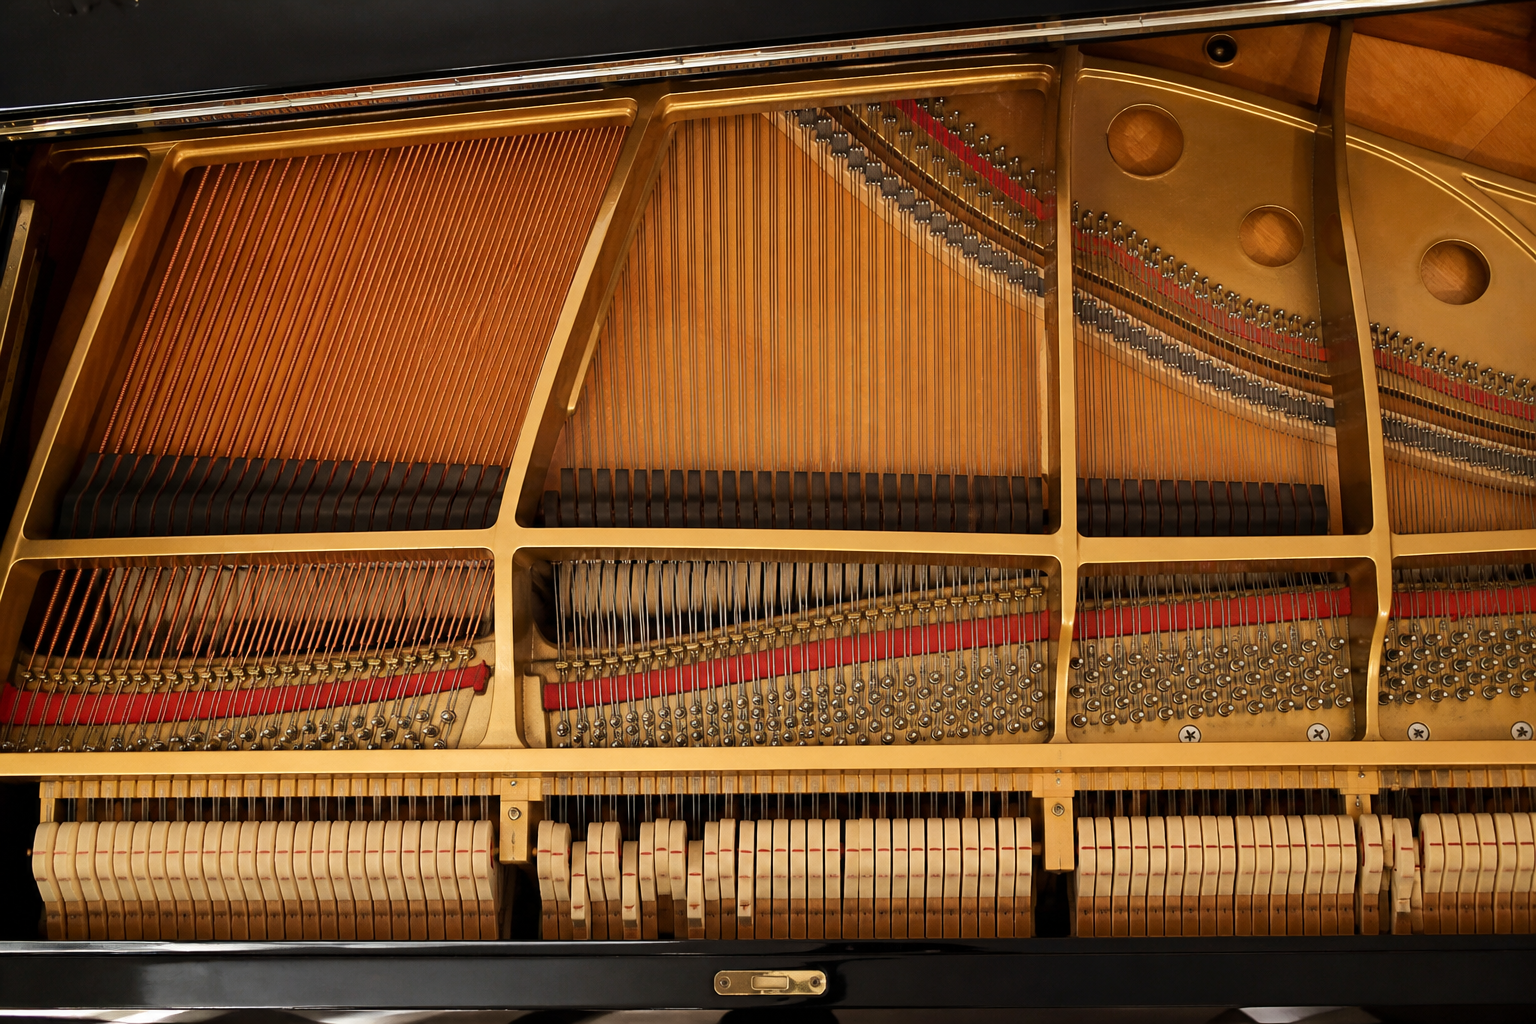
\includegraphics[width=0.58\linewidth]{images/book4/ai/b4-06-grand-piano-strings.png}

{\small Di dalam sebuah piano besar: sekitar dua ratus dawai baja dengan panjang dan tebal bertingkat, masing-masing dilaras oleh tegangannya ke nada dasar $c/2L$; dawai basnya dililit tembaga demi massanya.}
\end{omfigure}

\section{Soal: Piano, dari palu sampai papan resonansi}

\begin{problem}[{Soal akhir pekan --- sebuah dawai piano yang dibongkar: tegangan
dan kekakuannya, pukulan palunya dan harmonik yang dibuatnya,
jembatan yang membocorkan energinya ke papan resonansi, dan sebuah rel yang
mengemban persamaan yang sama}]
\label{pb:b2:waves-on-strings:1}

\medskip
\noindent\textbf{Bagian I --- Dawainya.}
Dawai A$_4$ sebuah piano (\qty{440}{Hz}): baja, $E = \qty{200}{GPa}$, $\rho =
\qty{7800}{kg/m^3}$, diameter $d = \qty{1.0}{mm}$, panjang berbunyi $L =
\qty{38}{cm}$. Setiap nada di atas basnya mempunyai tiga dawai semacam itu; pianonya
mempunyai $230$ dawai.
\begin{enumerate}
  \item Rapat massa linear, kelajuan gelombang dan tegangan dawainya.
  \item Tegangan tarik dalam kawatnya; kawatnya putus pada \qty{2.0}{GPa}:
        margin keselamatannya, dan mengapa putaran terakhir sang penala
        adalah yang berbahaya.
  \item Perkirakanlah tegangan total pada rangkanya, dengan mengambil semua dawainya
        pada tegangan yang sama.
  \item Dawai terendahnya (A$_0$, \qty{27.5}{Hz}) sepanjang \qty{1.9}{m}; seandainya ia
        kawat baja polos pada tegangan yang sama, $\mu$ berapa dan
        diameter berapa yang dituntutnya? Ia sesungguhnya inti baja yang dililit
        tembaga: jelaskanlah.
  \item Ragam dawai A$_4$: frekuensi delapan harmonik
        pertamanya; mana yang terletak pada selang yang selaras dengan nada
        dasarnya (oktaf, kuint, kuart, terts besar) dan mana yang
        tidak?
  \item Dawainya bergetar pada nada dasarnya dengan amplitudo
        \qty{0.50}{mm} di perutnya: energi yang tersimpan (energi sebuah
        ragam adalah $\tfrac14\mu L\omega^2A^2$).
  \item Tuliskanlah nada dasarnya sebagai jumlah dua gelombang berjalan; berikanlah
        amplitudonya dan daya rerata yang diemban masing-masing.
\end{enumerate}

\medskip
\noindent\textbf{Bagian II --- Palunya.}
Palunya memukul dawainya di $x_0 = L/8$, memberinya, pada $t = 0$, sebuah
kecepatan $v_0$ pada penggal pendek selebar $w$ di sekitar $x_0$ tanpa
simpangan.
\begin{enumerate}[resume]
  \item Tuliskanlah penyelesaian umumnya $y = \sum_nB_n\sin(n\pi x/L)\sin(\omega_nt)$
        lalu tunjukkanlah, dengan memakai keortogonalan sinusnya, bahwa $B_n =
        \dfrac{2}{L\omega_n}\int_0^L\dot y(x, 0)\sin\dfrac{n\pi x}L\,\dd x$.
  \item Untuk pukulan sempit ($w \ll L/n$), tunjukkanlah $B_n \approx \dfrac{2v_0w}
        {L\omega_n}\sin\dfrac{n\pi x_0}{L}$.
  \item Harmonik mana yang lenyap untuk $x_0 = L/8$? Mengapa pembuat piano
        memukul dekat $L/7$ sampai $L/8$ (lihatlah pertanyaan 5)?
  \item Lukiskanlah geraknya dalam gambaran gelombang berjalan: apa yang
        berangkat dari titik yang dipukul, apa yang terjadi di kedua ujungnya, dan sesudah
        waktu berapa keadaan awalnya berulang.
  \item Dawai sungguhan sedikit kaku: ragamnya adalah $f_n = nf_1
        \sqrt{1 + Bn^2}$ dengan $B = \pi^3Ed^4/(64TL^2)$ (diterima tanpa bukti). Hitunglah
        $B$ dan penajaman harmonik kedelapannya, dalam persen dan
        dalam sen (\qty{1}{sen} = nisbah frekuensi $2^{1/1200}$).
  \item Mengapa penala piano ``meregangkan'' oktafnya (melaras nada tinggi
        sedikit lebih tajam)?
\end{enumerate}

\medskip
\noindent\textbf{Bagian III --- Jembatan dan papan resonansi.}
Dawainya melintasi sebuah jembatan yang dilekatkan pada papan resonansi; papan resonansinya
berperilaku, di jembatannya, seperti tali berimpedansi $Z_b = \qty{2000}{kg/s}$.
\begin{enumerate}[resume]
  \item Impedansi $Z_s$ dawainya; koefisien pemantulan amplitudo
        di jembatannya.
  \item Bagian energi gelombangnya yang diteruskan ke papan resonansi pada
        setiap pemantulan.
  \item Jumlah pemantulan tiap sekon di jembatannya; simpulkanlah tetapan
        waktu peluruhan energinya dan waktu bagi bunyinya untuk turun
        \qty{60}{dB} (faktor $10^6$ dalam energi).
  \item Daya yang bocor ke papan resonansinya tepat sesudah pukulan
        pertanyaan 6; bandingkanlah dengan daya percakapan yang tenang,
        sekitar \qty{1e-5}{W} bunyi.
  \item Mengapa sebuah dawai sendirian hampir tak terdengar, dan apa yang
        dilakukan papan resonansinya terhadap itu? (Pikirkanlah impedansi udara,
        $\rho c \approx \qty{400}{kg.m^{-2}.s^{-1}}$, yang dilihat lewat permukaan
        kecil dibandingkan permukaan besar.)
  \item Dengan peredamnya terangkat, dawai A$_3$ (\qty{220}{Hz}) mulai
        berbunyi ketika A$_4$ dimainkan: mengapa?
  \item Seorang pembuat piano menginginkan bunyi yang bertahan lebih lama: haruskah $Z_b$ dinaikkan atau
        diturunkan, dan apa yang hilang?
\end{enumerate}

\medskip
\noindent\textbf{Bagian IV --- Rel.}
Sebuah rel baja ($E = \qty{200}{GPa}$, $\rho = \qty{7800}{kg/m^3}$, penampang
\qty{70}{cm^2}).
\begin{enumerate}[resume]
  \item Kelajuan gelombang mampatan; waktu bagi bunyi sebuah kereta untuk
        menempuh \qty{5}{km} sepanjang rel dan lewat udara.
  \item Sebuah pukulan palu mengirimkan pulsa mampatan menyusuri penggal rel
        \qty{25}{m} yang berujung bebas: waktu bagi gemanya; gemanya berupa
        mampatan atau peregangan?
  \item Sebuah pemeriksa ultrasonik \qty{2}{MHz} mencari retakan: panjang gelombangnya dalam
        baja; koefisien pemantulan amplitudo pada retakan baja--udara
        (impedansi udara $\qty{400}{kg.m^{-2}.s^{-1}}$); mengapa retakan
        tipis terlihat begitu jelas.
  \item Gempa bumi: dalam batuan, gelombang mampatan (P) berjalan dengan
        \qty{6.0}{km/s} dan gelombang geser (S) dengan \qty{3.5}{km/s}. Sebuah stasiun
        mencatat gelombang S \qty{20}{s} sesudah gelombang P: jarak ke
        sumbernya.
  \item Dalam satu tabel, kumpulkanlah kelima kelajuan gelombang soal ini
        (tali, rel, batuan P, batuan S, udara) beserta kekakuan dan
        kelembaman yang menetapkan masing-masingnya.
\end{enumerate}
\end{problem}
